\documentclass{article}

\usepackage{graphicx}
\usepackage[table,xcdraw]{xcolor}
\usepackage{listings}
\usepackage{indentfirst}
\usepackage[a4paper, total={6in, 8in}]{geometry}
\usepackage{hyperref}
\usepackage{fancyhdr}
\usepackage{xepersian}

\settextfont{B Nazanin}
\setlatintextfont{Times New Roman}

\begin{document}


%title page%
\begin{titlepage}
	\begin{center}
		\textbf{ \Huge{به نام خدا}}	
		\vspace{0.2cm}
		
		
\includegraphics[width=0.4\textwidth]{sharif.png}\\
		\vspace{0.2cm}
		\textbf{ \Huge{آزمایش شماره 8}}\\
		\vspace{0.25cm}
		\textbf{ \Large{آز معماری - دکتر سربازی آزاد}}
		\vspace{0.2cm}
		
		
		\large \textbf{دانشکده مهندسی کامپیوتر}\\\vspace{0.1cm}
		\large   دانشگاه صنعتی شریف\\\vspace{0.2cm}
		\large   ﻧﯿﻢ‌سال اول ۰۰-۰۱ \\\vspace{0.10cm}
		\large{\href{mailto:a.h.hadian@gmail.com}{امیرحسین هادیان - ۹۷۱۰۲۶۰۹}}\\
		\large{\href{mailto:mofayezi.m@gmail.com}{محمدرضا مفیضی - ۹۸۱۰۶۰۵۹}}\\
		\large{\href{mailto:a.hatam008@gmail.com}{علی حاتمی تاجیک - ۹۸۱۰۱۳۸۵}}\\
	\end{center}
\end{titlepage}
%title page%

\newpage

%pages header
\pagestyle{fancy}
\fancyhf{}
\fancyfoot{}
\setlength{\headheight}{59pt}
\cfoot{\thepage}
\lhead{آزمایش شماره 8}
\rhead{
\includegraphics[width=0.1\textwidth]{sharif.png}\\
		دانشکده مهندسی کامپیوتر
}
\chead{آز معماری}
%pages header

\section{هدف}
هدف این آزمایش پیاده‌سازی مدار کنترل کامپیوتر ساخته شده در آزمایش‌های قبل به صورت ریزبرنامه‌پذیر است.

\section{طراحی}
\subsection{مدار کنترلی}
برای طراحی مدار کنترلر به صورت ریزبرنامه‌‌پذیر ابتدا باید میکرو اینستراکشن‌ها را طراحی کنیم که شرح آن به شکل زیر است:
ابتدا دستور را در ثبات لود می‌کنیم.(\lr{fetch})
سپس شمارنده دستور را یکی زیاد می‌کنیم تا در مرحله بعدی آن را لود کنیم و اگر دستور پرشی باشد، مقدار آدرس پرش در شمارنده دستور لود می‌شود و سپس دستور مور نظر لود خواهد شد.
سپس با بررسی بیت‌های دستور از بیت پر‌ارزش، نوع دستور را تشخیص می‌دهیم و سیگنال‌های کنترلی درست را ارسال می‌کنیم که این عمل تشخیص دستور با استفاده از میکرو آپکود‌ها و معماری سیستم کنترلی موجود در صورت آزمایش صورت می‌گیرد.
جدول دستور‌های میکرو اینستراکشن که در حافظه به صورت ایستا ذخیره شده است در جدول \ref{micro-instructions} آمده است.

\begin{table}[]
\begin{latin}
\resizebox{\textwidth}{!}{%
\begin{tabular}{|c|c|l|c|
>{\columncolor[HTML]{D9D9D9}}c |
>{\columncolor[HTML]{D9D9D9}}c |c|c|c|c|
>{\columncolor[HTML]{D9D9D9}}c |
>{\columncolor[HTML]{D9D9D9}}c |
>{\columncolor[HTML]{D9D9D9}}c |
>{\columncolor[HTML]{D9D9D9}}c |c|c|c|c|}
\hline
command &
  address &
  \multicolumn{1}{c|}{hex address} &
  binary address &
  micro-opcode &
  enable &
  s\_select &
  d\_select &
  op &
  load\_sr &
  OE1 &
  OE2 &
  WE &
  extra &
  load\_IR &
  enable\_counter &
  load\_pc &
  extra \\ \hline
no operation            & 0  &    & 00000000 & 000 & 0 & 0 & 0 & 0 & 0 & 0 & 0 & 0 & 0 & 0 & 0 & 0 & 0 \\ \hline
fetch - load IR         & 1  & 01 & 00000001 & 000 & 0 & 0 & 0 & 0 & 0 & 1 & 1 & 1 & 0 & 1 & 0 & 0 & 0 \\ \hline
fetch - count pc        & 2  & 02 & 00000010 & 000 & 0 & 0 & 0 & 0 & 0 & 1 & 1 & 1 & 0 & 0 & 1 & 0 & 0 \\ \hline
check jump instrucntion & 3  & 03 & 00000011 & 001 & 0 & 0 & 0 & 0 & 0 & 0 & 0 & 0 & 0 & 1 & 1 & 1 & 1 \\ \hline
check mem instruction   & 4  & 04 & 00000100 & 010 & 0 & 0 & 0 & 0 & 0 & 0 & 0 & 0 & 0 & 1 & 0 & 1 & 0 \\ \hline
alu - check sub         & 5  & 05 & 00000101 & 011 & 0 & 0 & 0 & 0 & 0 & 0 & 0 & 0 & 0 & 1 & 0 & 0 & 0 \\ \hline
add                     & 6  & 06 & 00000110 & 000 & 1 & 0 & 0 & 0 & 1 & 1 & 1 & 1 & 0 & 0 & 0 & 0 & 0 \\ \hline
jump to fetch           & 7  & 07 & 00000111 & 111 & 0 & 0 & 0 & 0 & 0 & 0 & 0 & 0 & 0 & 0 & 0 & 0 & 1 \\ \hline
sub                     & 8  & 08 & 00001000 & 000 & 1 & 0 & 0 & 1 & 1 & 1 & 1 & 1 & 0 & 0 & 0 & 0 & 0 \\ \hline
jump to fetch           & 9  & 09 & 00001001 & 111 & 0 & 0 & 0 & 0 & 0 & 0 & 0 & 0 & 0 & 0 & 0 & 0 & 1 \\ \hline
memory - check store    & 10 & 0A & 00001010 & 011 & 0 & 0 & 0 & 0 & 0 & 0 & 0 & 0 & 0 & 1 & 1 & 0 & 1 \\ \hline
memory load             & 11 & 0B & 00001011 & 000 & 1 & 0 & 1 & 0 & 0 & 0 & 0 & 1 & 0 & 0 & 0 & 0 & 0 \\ \hline
jump to fetch           & 12 & 0C & 00001100 & 111 & 0 & 0 & 0 & 0 & 0 & 0 & 0 & 0 & 0 & 0 & 0 & 0 & 1 \\ \hline
memory store            & 13 & 0D & 00001101 & 000 & 0 & 1 & 0 & 0 & 0 & 1 & 1 & 0 & 0 & 0 & 0 & 0 & 0 \\ \hline
jump to fetch           & 14 & 0E & 00001110 & 111 & 0 & 0 & 0 & 0 & 0 & 0 & 0 & 0 & 0 & 0 & 0 & 0 & 1 \\ \hline
jump - check o , always & 15 & 0F & 00001111 & 010 & 0 & 0 & 0 & 0 & 0 & 0 & 0 & 0 & 1 & 0 & 1 & 0 & 1 \\ \hline
jump - check s          & 16 & 10 & 00010000 & 011 & 0 & 0 & 0 & 0 & 0 & 0 & 0 & 0 & 1 & 0 & 0 & 1 & 1 \\ \hline
jump if z = 1           & 17 & 11 & 00010001 & 100 & 0 & 0 & 0 & 0 & 0 & 0 & 0 & 0 & 1 & 1 & 0 & 0 & 0 \\ \hline
jump to fetch           & 18 & 12 & 00010010 & 111 & 0 & 0 & 0 & 0 & 0 & 0 & 0 & 0 & 0 & 0 & 0 & 0 & 1 \\ \hline
jump if s = 1           & 19 & 13 & 00010011 & 101 & 0 & 0 & 0 & 0 & 0 & 0 & 0 & 0 & 1 & 1 & 0 & 0 & 0 \\ \hline
jump to fetch           & 20 & 14 & 00010100 & 111 & 0 & 0 & 0 & 0 & 0 & 0 & 0 & 0 & 0 & 0 & 0 & 0 & 1 \\ \hline
jump - check always     & 21 & 15 & 00010101 & 011 & 0 & 0 & 0 & 0 & 0 & 0 & 0 & 0 & 1 & 1 & 0 & 0 & 0 \\ \hline
jump if o = 1           & 22 & 16 & 00010110 & 110 & 0 & 0 & 0 & 0 & 0 & 0 & 0 & 0 & 1 & 1 & 0 & 0 & 0 \\ \hline
jump to fetch           & 23 & 17 & 00010111 & 111 & 0 & 0 & 0 & 0 & 0 & 0 & 0 & 0 & 0 & 0 & 0 & 0 & 1 \\ \hline
always jump             & 24 & 18 & 00011000 & 000 & 0 & 0 & 0 & 0 & 0 & 1 & 1 & 1 & 0 & 0 & 0 & 1 & 0 \\ \hline
jump to fetch           & 25 & 19 & 00011001 & 111 & 0 & 0 & 0 & 0 & 0 & 0 & 0 & 0 & 0 & 0 & 0 & 0 & 1 \\ \hline
\end{tabular}%
}
\end{latin}
\caption{میکروایسنتراکشن‌ها}
\label{micro-instructions}
\end{table}

برای طراحی فیزیک این قسمت از طراحی پیشنهادی موجود در صورت آزمایش استفاده شد. طول میکرو اینستراکشن‌ها با توجه به تعداد سیگنال‌های کنترلی ۱۶ بیت شد که البته ۲ بیت آن رزرو است و بعدا می‌تواند مورد استفاده قرار گیرد.
به علت اینکه حافظه ۱۶ بیتی در پروتئوس نداشتیم، از دو حافظه ۸ بیتی برای ذخیره میکرو اینستراکشن‌ها استفاده کردیم.
تصویر مدار کنترل در شکل \ref{fig:cu} آمده است. 

\begin{figure}
	\resizebox{\textwidth}{!}{%
	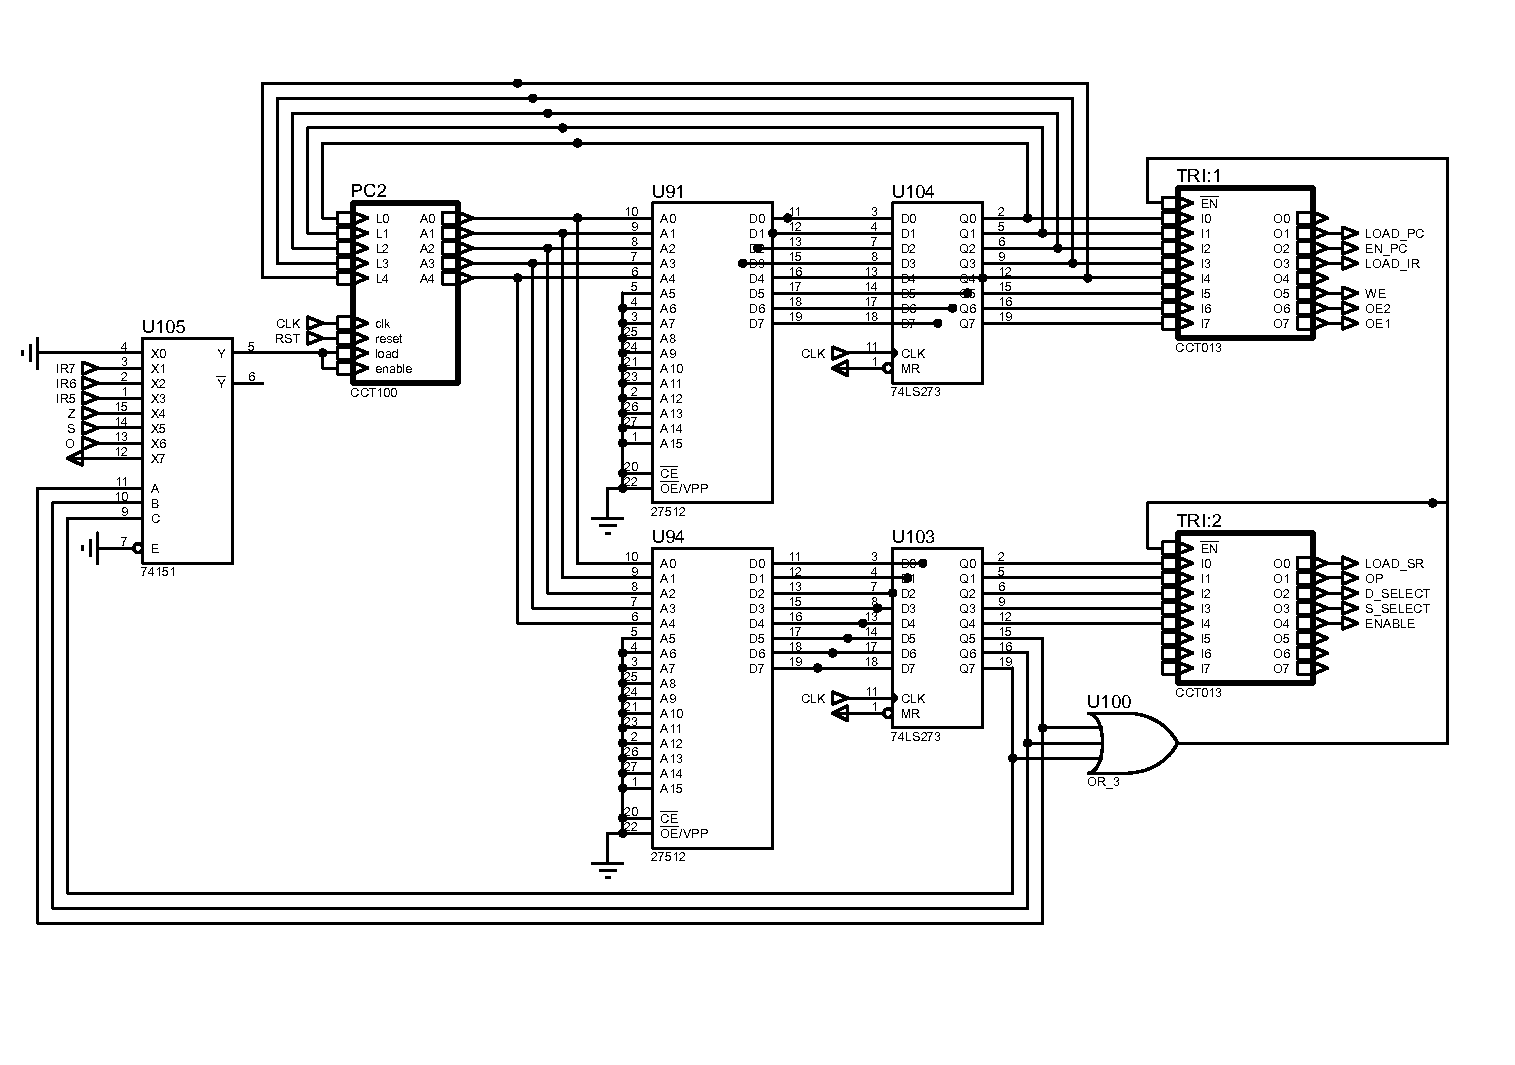
\includegraphics{./graphics/cu}
	}
	\caption{مدار کنترلی}
	\label{fig:cu}
\end{figure}

\subsection{تغییرات انجام شده}
در این آزمایش بخش کنترلی به طور کامل با ریز معماری اجرا کننده ریز دستورات جایگزین شده ولی ورودی‌ها همچنان مثل آزمایش قبل \lr{IR} و خروجی‌ها سیگنال‌های کنترلی مورد نیاز در مدار هستند.
از طرفی چون در بعضی حالات ریز دستورات، سینگال‌های کنترلی به \lr{z} تغییر پیدا می‌کنند (با استفاده از بافر سه حالته)، در ورودی رجیسترها و بخش‌هایی از مدار که از این سیگنال ها استفاده می‌کنند از \lr{and} این سیگنال‌ها با کلاک استفاده شده تا مقدار \lr{z} عملکرد این بخش‌ها را خراب نکند.
از آنجایی که در ریز دستورات به خود دستور دسترسی نداریم، با تعیین سیگنال کنترلی یک مالتی پلکسر مشخص می‌کنیم که مبدا و مقصد در \lr{ALU} از دستور خوانده شود و یا مقدار ثابت از پیش تعیین شده باشد.

\section{تست}
برای بررسی درستی عملکرد سیستم، برنامه اول آزمایش قبل (جمع 10 جمله اول از سری فیبوناچی) را روی ماشین اجرا کردیم که خروجی آن به صورت شکل \ref{fig:test} است. حاصل یعنی عدد ۸۸ به صورت باینری در رجیستر \lr{R0} (همان \lr{A}) نشان داده شده است (که از آدرس صفر حافظه خوانده شده است).

\begin{figure}
	\resizebox{\textwidth}{!}{%
	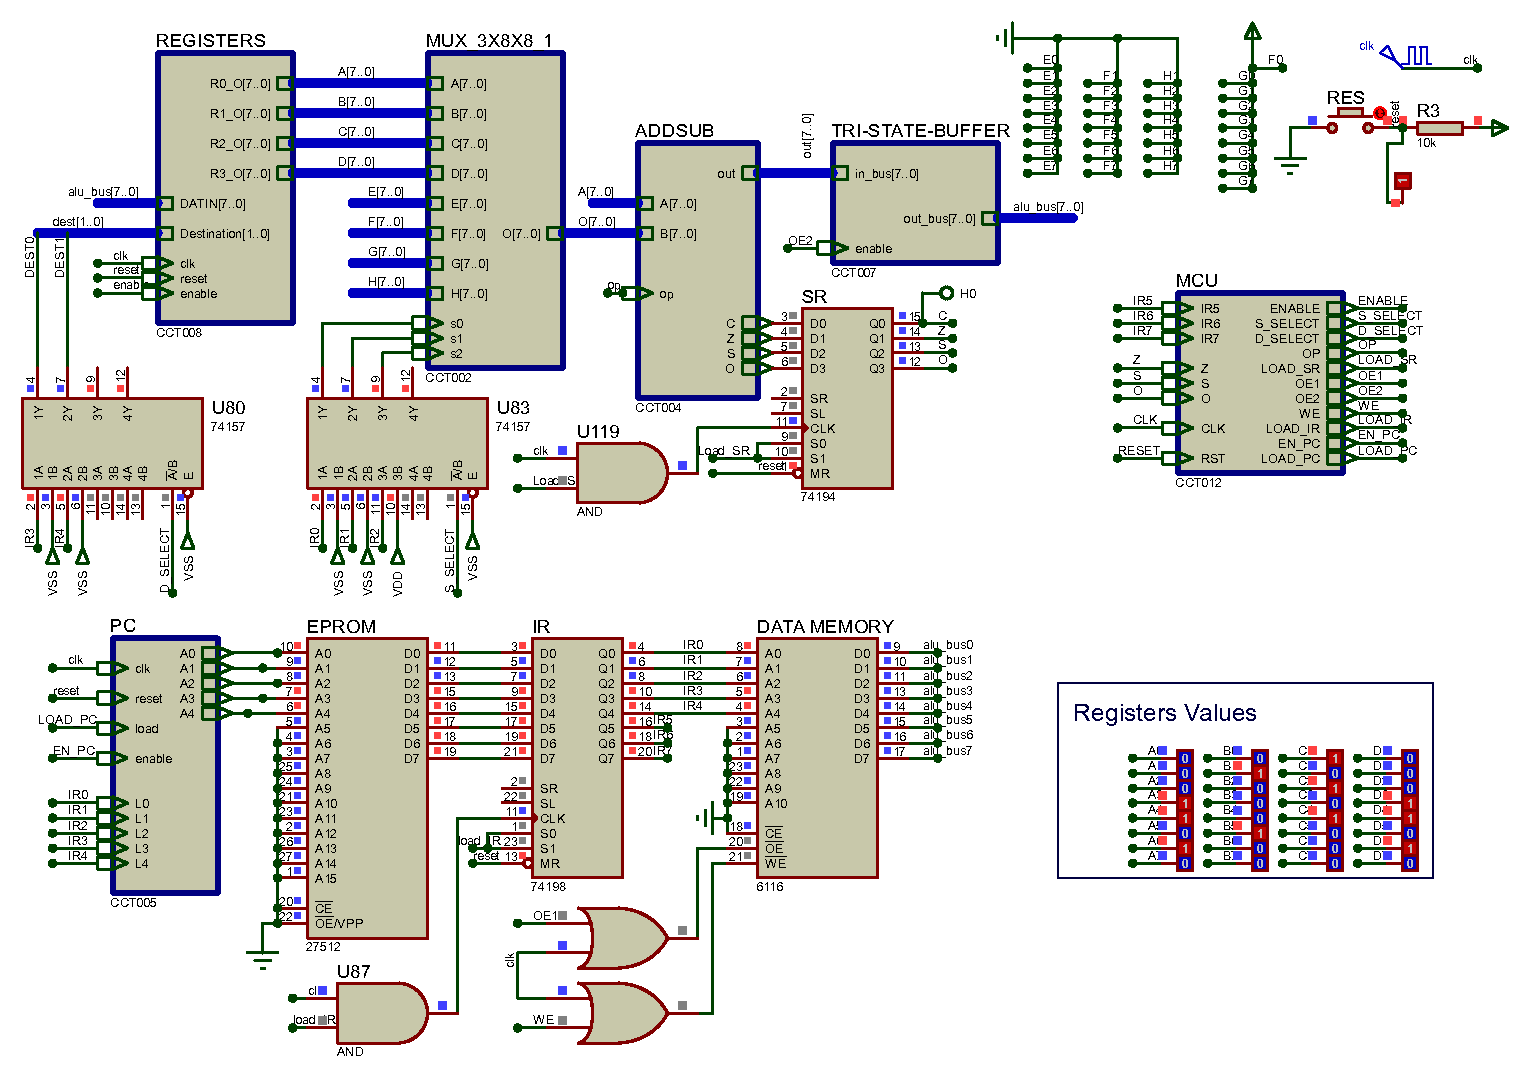
\includegraphics{./graphics/test}
	}
	\caption{تست}
	\label{fig:test}
\end{figure}
\end{document}
